\section{Agents}

As mentioned before, there are two main types of agents: generators and testers.
Generators extend or modify an existing counterpoint line to create a new partial composition.
Testers examine a counterpoint line (usually at the current end) to see if it acceptable.
Generators and testers work together through a feedback loop to create valid compositions.

\begin{figure}[h]
\centering
	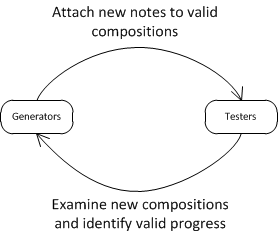
\includegraphics[keepaspectratio=true]{generator-and-tester-dynamic.png}
\caption{The generator and tester agent dynamic}
\end{figure}

Agents can also be divided by the ruleset they help implement.
For example, implementing florid counterpoint involves six rulesets: general rules, four sets of species specific rules, and species boundary rules.

Regarding counterpoint, tester agents have another division: hard rules (mandatory) and soft rules (optional, but preferred).
These rules were derived from the descriptions in ``Modal Counterpoint: Renaissance Style'' by Peter Schubert (add better citation later).

\subsection{General Counterpoint Rules}

\paragraph{Generators}
The counterpoint species determines the start and duration of a note, so there is no reasonable way to generate notes outside of the context of a species.
Thus, no generator agents fall within the General Counterpoint Rules grouping.

\paragraph{Testers}
\subparagraph{Hard Rules}
	\begin{enumerate}
		\item No augmented or diminished skips. No skips larger than a sixth unless it is an octave.
					Implementation involves checking the current and previous notes to build the interval and test it.

		\item No outlines of augmented fourths. No outlines of diminished fifths unless completely filled in and followed by an opposite direction step.
					An interval is outlined if the local high and low points of a line form that interval.
					Implementation involves moving back from the current note to find the last complete segment with a low and a high, and then testing that interval.
					Testing the segment ending in the current note does not serve much purpose because we don't know if it will be a local high or low yet. The exception is the last note of the composition.

		\item The first and last notes of each part (\emph{cantus firmus} and counterpoint) must form a perfect consonant interval, i.e. a perfect unison, fifth, octave, or occasionaly a twelth.
					This agent would simply return a test pass for interior notes.

	\end{enumerate}
\subparagraph{Soft Rules}
	\begin{enumerate}
		\item Use steps, movement to adjacent notes, more than skips, movement to non-adjacent notes. Specific ratios are usually determined by species, but the general agent would aim for a minimum rate.
		
		\item Avoid skips of a major sixth and descending minor sixths.

		\item Precede or follow a skip by a step in the opposite direction. Examine the current note and the two preceding notes in order to check validity of the first preceding note.

		\item Do not use more than two skips in sequence. Examine the current note and the three preceding notes to check if all three intervals are skips.

		\item Two successive skips in the same direction should be small skips. A `small' interval is a fourth or smaller.

		\item In a sequence of skips and steps in the same direction, larger intervals should be below smaller ones.
					Move back from the current note, testing intervals along the way, while motion is in the same direction.

		\item Do not skip both to and from a high or low point. This is a more specific version of soft rule 3 that focuses specifically on local highs and lows.
					Scan back to the previous high or low and check if it is bounded by skips.

		\item Accidental $B\flat$s, i.e. ones that occur when $B\flat$ is not in the mode, should be followed by descending motion.
					Check if the previous note is a accidental $B\flat$. If so, check whether the current note descended from it.

	\end{enumerate}

\subsection{First Species Counterpoint Rules}

agents for first species rules

\paragraph{Generators}
First species involves matching each note of the \emph{cantus firmus} with one simultaneous note of counterpoint. These are always whole notes.
The first species generator attaches a randomly selected note from the two octaves either above or below the \emph{cantus firmus} (the two lines never cross) to the end of an existing composition.
The attached note will always be a whole note and will have at most one accidental.
\paragraph{Testers}
\subparagraph{Hard Rules}
	\begin{enumerate}
		\item All downbeats, which in the case of first species is all beats, must be consonant with the \emph{cantus firmus}. 
					Consonant intervals are unisons, thrids, fifths, sixths, octaves, and their compounds.
					This agent just checks the current note with the corresponding note in the \emph{cantus firmus}.

		\item Enter perfect intervals only by contrary motion, in which voices move in opposite directions, or oblique motion, in which one voice does not move.
					If the current vertial interval is perfect, then the agent examines the motion from the previous notes in both voices.

		\item If the \emph{cantus firmus} repeated a note, the counterpoint may not also repeat a note. This refers specifically to adjacent repeated notes.
					An exception is that octave skips in the counterpoint are allowed if the \emph{cantus firmus} is stationary.

		\item The counterpoint and the \emph{cantus firmus} can move in parallel (same intervals) for at most four notes. Because of rule 2, only thirds and sixths are allowed for parallel motion.

		\item Skips must be less than half of all melodic motions.
					This agent scans back through the line and computes the skip to step ratio.

		\item Do not directly repeat a combination; sequential repitiions are limited to two. A combination is a subsequence (of both voices) at least two notes long.
					Direct repetition involves exactly repeating this subsequence immediately; exact repetition is allowed if at least two whole notes of other material is between the repetitions.
					Sequential repeition involves transposing, moving up or down, the combination and playing this transposition. 
					The limit of two repetitions means this sequence can actually occur three times in a row (original and two repetitions).

					There are two relevant sequences here: the sequence of vertical intervals and the sequence of motion interval pairs. 
					Finding direct repetitions involves identifying a subsequence (across both sequences) involving the current note that is repeated elsewhere and checking that these repetitions are separated enough.
					Finding sequential repetitions involves indentifying a repeated subsequence in the vertical intervals that corresponds to a one element shorter subsequence in the motion intervals with repetitions
						separated by a parallel interval.

					Since we only need to check how the most recently added note, which is the only untested note, changes things, we only need to check subsequences that end on the current note.
					This makes the check quadratic instead of exponential.
	\end{enumerate}
\subparagraph{Soft Rules}
	\begin{itemize}
		\item Avoid using more that two perfect vertical intervals in a row.
		\item Avoid vertical unisons except on the first and last notes.
		\item Avoid simultaneous skips. It is ok if both voices are skipping by a third.
		\item Avoid the vertical interval being larger than a twelfth.
		\item Try to change direction after a large (fifth or more) skip and move by a step.
		\item Try to connect extreme points (local highs and lows) with smooth, stepwise motion. This filling can occur before or after a skip.
		\item Try to cover a whole octave every 10 to 20 \emph{cantus firmus} notes. Octave skips do not reset the counter.
	\end{itemize}
